% Complete Chapter 1, original PDF 11-20 / printed 1-10.
% block: introduction-heading page:11 type:chapter
\clearpage\setcounter{section}{0}
\section{{引言}}\label{chap:introduction}

% block: feec-framework page:11 type:ordinary-paragraph
{有限元外微积分, 简称 FEEC, 是设计和理解求解多种偏微分方程数值解的有限元方法的一种理论途径. 有限元方法本身是计算科学与工程中最重要的技术之一. 它的成功在很大程度上得益于过去 50 年间发展起来的数学框架, 这一框架使严格的误差分析以及对不同有限元方法和计算性质的理解成为可能. 传统上, 这一框架主要基于泛函分析的语言和工具. FEEC 又引入了拓扑和同调代数的工具. 更具体地说, FEEC 在离散层次捕捉 de Rham 上同调和 Hodge 理论的本质结构, 并将连续结构与离散结构联系起来, 从而获得稳定且收敛的有限元离散化.}

% block: motivating-failures page:11 type:ordinary-paragraph
{\emergencystretch=1em
{接下来的各章将介绍必要的同调代数和泛函分析背景知识, 然后利用这些知识发展 FEEC, 并将其应用于不同情境. 不过, 读者或许希望先了解一些动机. 我们为什么需要为有限元建立一套精细的新理论? 毕竟, 有限元方法在许多应用中表现出色. 本章将展示一些简单的数值例子: 标准有限元方法在这些例子中彻底失效, 而经过精心构造以保留相应 PDE 问题关键结构的、更精巧的有限元却能解决问题.}
\par}

% block: poisson-model-intro page:11 type:ordinary-paragraph
{首先回顾有限元方法的一些经典理论, 为后文作准备. 有限元最简单的应用情形是 Poisson 方程 Dirichlet 问题的数值求解. 给定 $\mathbb R^n$ 中区域 $\Omega$ 上的实值函数 $f$, 我们寻求满足下式的函数 $u$:}

% block: poisson-strong-form page:11 type:equation
\[
-\Delta u=f\text{{ 在 }}\Omega,\qquad u=0\text{{ 在 }}\partial\Omega.
\]

% block: poisson-weak-intro page:11 type:ordinary-paragraph
{有限元方法并不从这一强表述出发, 而是从该边值问题的弱表述出发. 我们在 Sobolev 空间 $\mathring H^1(\Omega)$ 中寻求解 $u$, 这个空间由一阶偏导数也属于 $L^2(\Omega)$ 且在 $\partial\Omega$ 上为零的 $L^2(\Omega)$ 函数组成. 解由要求下式成立来确定:}

% block: poisson-weak-equation page:11 type:equation
\begin{equation}\label{eq:poisson-weak-form}
\int_\Omega\operatorname{grad}u\cdot\operatorname{grad}v\,dx=\int_\Omega fv\,dx
\end{equation}

% block: poisson-well-posedness page:12 type:ordinary-paragraph
{对检验空间 $\mathring H^1(\Omega)$ 中的所有函数 $v$ 成立 (在本例中, 检验空间与寻求 $u$ 的试探空间相同). 该方程由原 Poisson 方程乘以检验函数 $v$, 再在区域 $\Omega$ 上作分部积分得到. 该问题的弱表述是适定的, 即对任意 $f$ (属于 $L^2(\Omega)$, 甚至属于对偶 Sobolev 空间 $H^{-1}(\Omega)=\mathring H^1(\Omega)'$), 都存在唯一弱解 $u$, 并且作为 $H^1$ 中的元素, 它连续依赖于 $L^2$ 或 $H^{-1}$ 中的 $f$.}

% block: galerkin-subspace page:12 type:ordinary-paragraph
{为计算近似解 $u_h$, 我们先考虑包含有限元方法在内的 Galerkin 方法. Galerkin 方法要求指定 $\mathring H^1(\Omega)$ 的一个有限维子空间 $V_h$, 在离散层次同时用作试探空间和检验空间. 因此, 我们通过要求弱方程 \eqref{eq:poisson-weak-form} 对属于 $V_h$ 的检验函数 $v$ 成立, 来寻求近似解 $u_h\in V_h$:}

% block: poisson-galerkin-equation page:12 type:equation
\begin{equation}\label{eq:poisson-galerkin-form}
\int_\Omega\operatorname{grad}u_h\cdot\operatorname{grad}v\,dx=\int_\Omega fv\,dx,\qquad v\in V_h.
\end{equation}

% block: stiffness-and-load page:12 type:ordinary-paragraph
{这是一个维数等于 $\dim V_h$ 的有限维线性方程组. 为计算其解, 需要指定 $V_h$ 的一组基 $\phi_i$, 计算以 $\int_\Omega\operatorname{grad}\phi_j\cdot\operatorname{grad}\phi_i\,dx$ 为元素的刚度矩阵和以 $\int_\Omega f\phi_i\,dx$ 为元素的载荷向量, 然后求解所得矩阵方程; 其解给出 $u_h$ 在所选基下的系数. 在这个简单情形下, 刚度矩阵对称正定, 因而近似解唯一确定. 注意, 计算 Galerkin 解的代价由两部分组成: 计算每个基元素对应的刚度矩阵和载荷向量元素的代价, 以及求解所得线性方程组的代价.}

% block: poincare-error-estimate-intro page:12 type:ordinary-paragraph
{Galerkin 方法的解不仅唯一确定且可计算, 而且其误差估计也容易导出. 在当前情形下, 只需调用 Poincaré 不等式}

% block: poincare-inequality page:12 type:equation
\[
\|w\|_{H^1}\le c\|\operatorname{grad}w\|_{L^2},\qquad w\in\mathring H^1,
\]

% block: hilbert-projection-quasioptimality page:12 type:ordinary-paragraph
{其中常数 $c$ 只依赖于区域 $\Omega$. 因而 \eqref{eq:poisson-weak-form} 左端的双线性型在 $\mathring H^1$ 上定义一个内积, 其范数与 $H^1$ 内积所对应的范数等价. 因此, 可以应用 Hilbert 投影定理证明该解在 $H^1$ 范数下拟最优:}

% block: galerkin-quasioptimality page:12 type:equation
\begin{equation}\label{eq:galerkin-quasioptimality}
\|u-u_h\|_{H^1}\le c\inf_{v\in V_h}\|u-v\|_{H^1},
\end{equation}

% block: quasioptimality-constant page:12 type:ordinary-paragraph
{其中的常数仍为同一个 $c$, 与 $f$、$u$ 以及子空间 $V_h$ 的选择无关.}

% block: lagrange-piecewise-linears page:12 type:ordinary-paragraph
{有限元方法是一种 Galerkin 方法, 其中的 Galerkin 子空间 $V_h$ 是可高效计算的分片多项式空间 (更准确地说, 它可以通过 Section~\ref{sec:complete-polynomial-forms} 开头回顾的组装过程构造). 最简单的有限元是 Lagrange 分片线性元. 在二维情形下, 将区域 $\Omega$ 作三角剖分 (因此假设区域是多边形, 或用多边形逼近), 并令 $V_h$ 由在剖分的每个三角形上都是次数至多为 1 的多项式、且在 $\partial\Omega$ 上为零的所有连续函数组成, 就得到有限元空间. Figure~\ref{fig:annular-lagrange-basis} 展示了区域 $\Omega=(0,3)\times(0,3)\setminus[2/3,2]\times[3/4,2]$ 的一个相当粗的三角剖分, 共含 256 个三角形. 图的中间是一个满足 Dirichlet 边界条件的分片线性函数的例子.}

% block: annular-lagrange-basis-figure page:13 type:figure
\begin{figure}[H]\centering
\includegraphics[page=13,trim=106bp 573bp 56bp 62bp,clip,width=.9\linewidth]{../input/source/Finite Element Exterior Calculus.pdf}
\caption{{左: 环状多边形区域的三角剖分. 中: 一个分片线性函数. 右: 一个 Lagrange 基函数.}}\label{fig:annular-lagrange-basis}
\end{figure}

% block: local-basis-and-refinement page:13 type:ordinary-paragraph
{这个空间的维数等于三角剖分的内部顶点数, 它有一组方便的基, 称为 Lagrange 基: 每个基函数在唯一一个内部顶点处等于一, 在其余内部顶点处等于零, 如图的右侧所示. 这是一组局部基, 意指每个基函数的支集仅覆盖少数几个三角形. 因而, 刚度矩阵和载荷向量所需的积分可以很快算出, 且刚度矩阵高度稀疏 (当网格加密时, 渐近地每行平均只有七个非零元素). 因此有限元解可高效计算. 由 \eqref{eq:galerkin-quasioptimality}, 它在 $H^1(\Omega)$ 中的精度与该网格上最佳连续分片线性逼近的精度相当. 为提高有限元解的精度, 可以通过加密网格来扩充有限元空间. 也可以使用更高次的 Lagrange 有限元, 即把分片多项式的次数提高到某个 $d>1$. 将估计 \eqref{eq:galerkin-quasioptimality} 与逼近理论结合, 可保证当网格尺寸趋于 0 或单元次数趋于 $\infty$ 时, 误差趋于 0.}

% block: classical-theory-directions page:13 type:ordinary-paragraph
{我们用一个简单的模型问题说明了有限元方法的基本方面. 通常, 接下来会建立收敛阶及其对三角剖分和解正则性的依赖关系, 证明 $H^1$ 范数以外其他范数下的误差估计, 发展后验误差估计和自适应网格算法并分析其性能, 当然还会推广到其他问题. 这方面的论述可参见众多现有著作, 例如 \BookCite{21}、\BookCite{22}、\BookCite{31}、\BookCite{40}.}

% block: scalar-laplacian-eigenproblem page:13 type:ordinary-paragraph
{为了说明研究 FEEC 的动机, 我们很快将讨论一个使标准有限元途径失效的问题. 不过, 先继续讨论标准有限元方法, 但不再针对刚才的源问题, 而是针对 Laplacian 特征值问题. 标准有限元对这一问题同样十分成功, 并且有大量理论论证, 其中很大程度上依赖 Hilbert 空间中的谱理论 \BookCite{16}、\BookCite{18}. 仍使用 Figure~\ref{fig:annular-lagrange-basis} 中的区域, 我们寻求一面环状多边形鼓的基模和基频 (也可能是若干振型和频率). 也就是说, 要找到最小的 $\lambda\in\mathbb R$, 使得存在非零 $u:\Omega\to\mathbb R$ 满足}

% block: scalar-eigenproblem-equation page:13 type:equation
\begin{equation}\label{eq:scalar-laplacian-eigenproblem}
-\Delta u=\lambda u\text{{ 在 }}\Omega,\qquad u=0\text{{ 在 }}\partial\Omega.
\end{equation}

% block: discrete-scalar-eigenproblem-intro page:13 type:ordinary-paragraph
{转为弱表述并应用 Galerkin 方法, 就得到求 $\lambda_h\in\mathbb R$ 和非零 $u_h\in V_h$ 的离散特征值问题, 使得}

% block: discrete-scalar-eigenproblem page:13 type:equation
\[
\int_\Omega\operatorname{grad}u_h\cdot\operatorname{grad}v\,dx=\lambda_h\int_\Omega u_hv\,dx,\qquad v\in V_h.
\]

% block: scalar-eigenvalue-table page:14 type:table
\begin{table}[H]\centering
\caption{{Figure~\ref{fig:annular-lagrange-basis} 中区域上 Laplacian 的第一和第二特征值, 在给定网格的均匀加密网格上使用 1 次和 3 次 Lagrange 元计算. 精确到最接近的 0.001, 正确值为 9.190 和 11.166.}}\label{tab:scalar-laplacian-eigenvalues}
\begin{tabular}{r|rr|rr}\hline
&\multicolumn{2}{c|}{{1 次}}&\multicolumn{2}{c}{{3 次}}\\
{单元数}&$\lambda_1$&$\lambda_2$&$\lambda_1$&$\lambda_2$\\\hline
256&9.986&12.003&9.211&11.179\\
1,024&9.428&11.404&9.198&11.171\\
4,096&9.279&11.245&9.193&11.168\\
16,384&9.216&11.189&9.191&11.167\\
65,536&9.199&11.174&9.190&11.167\\
262,144&9.193&11.169&9.190&11.166\\\hline
\end{tabular}
\end{table}

% block: generalized-eigenvalue-solution page:14 type:ordinary-paragraph
{通过一组基, 这可以化为一个对称稀疏广义特征值问题: 其中一个矩阵是上面定义的刚度矩阵, 另一个是以类似方式、但使用方程右端出现的 $L^2$ 内积定义的质量矩阵. 这一矩阵广义特征值问题可用迭代方法高效求解, 例如用反幂法求基特征对, 或用 Krylov–Schur 迭代计算某个区间内的谱. 在理论方面, 可以证明当前情形下第一个特征函数 $u_h$ 满足形如 \eqref{eq:galerkin-quasioptimality} 的拟最优误差估计, 且特征值误差不超过特征函数误差平方的某个倍数. 清晰的论述可参见例如 \BookCite{18}, 其中也包括多于一个特征值的情形以及非单特征值所引起的复杂情况.}

% block: scalar-numerical-results page:14 type:ordinary-paragraph
{接下来用一些数值结果说明其表现. 对 Figure~\ref{fig:annular-lagrange-basis} 中含 256 个三角形的粗网格, 使用 Lagrange 线性有限元算出的基本特征值为 9.986, 所算基特征函数如 Figure~\ref{fig:annular-lagrange-basis} 中间所示. 鉴于网格很粗, 这些结果不太精确并不意外 (特征值误差约为 9\%). 不过, 通过加密网格和/或提高多项式次数, 可以将精度提高到所需程度. Table~\ref{tab:scalar-laplacian-eigenvalues} 给出 1 次和 3 次多项式下基本特征值和第二特征值的结果, 所用的一列网格由初始网格均匀加密得到. 用含 65,536 个三角形的分片线性元, 或含 1,024 个三角形的分片三次元, 基本特征值误差可控制在约 0.1\% 以内. Figure~\ref{fig:scalar-fundamental-mode} 展示了在含 65,536 个三角形的网格上用线性 Lagrange 元计算的基特征函数. 值得指出, 使用自适应加密, 可以用少得多的三角形达到这些均匀加密网格的精度, 不过本书不讨论这一方向.}

% block: vector-laplacian-model page:14 type:ordinary-paragraph
{现在考虑一个经典途径不足以处理、而 FEEC 能够解决的问题. 为此, 我们稍稍离开标量 Laplacian, 转而考虑向量 Laplacian, 即作用于向量场 $u:\Omega\to\mathbb R^2$ 的算子 $-\Delta=\operatorname{curl}\operatorname{curl}-\operatorname{grad}\operatorname{div}$. (由于处于二维, $\operatorname{curl}u$ 是标量函数, 而第二次应用 $\operatorname{curl}$ 将该标量函数映回向量场.) 因此考虑特征值问题}

% block: vector-laplacian-eigenproblem page:14 type:equation
\begin{equation}\label{eq:vector-laplacian-eigenproblem}
(\operatorname{curl}\operatorname{curl}-\operatorname{grad}\operatorname{div})u=\lambda u\text{{ 在 }}\Omega,\qquad u\cdot n=\operatorname{curl}u=0\text{{ 在 }}\partial\Omega.
\end{equation}

% block: scalar-fundamental-mode-figure page:15 type:figure
\begin{figure}[H]\centering
\includegraphics[page=15,trim=147bp 504bp 98bp 62bp,clip,width=.65\linewidth]{../input/source/Finite Element Exterior Calculus.pdf}
\caption{{在 65,536 个三角形上用分片线性元计算的基特征函数.}}\label{fig:scalar-fundamental-mode}
\end{figure}

% block: magnetic-boundary-spaces page:15 type:ordinary-paragraph
{这些边界条件因其在电磁学中的应用, 有时称为磁边界条件, 它们允许一种简单的弱表述. 定义空间 $\mathring H(\operatorname{div})$, 由散度属于 $L^2$ 且在边界上 $u\cdot n$ 为零的 $L^2$ 向量场组成; 再定义空间 $H(\operatorname{curl})$, 由旋度属于 $L^2$ 的 $L^2$ 向量场组成 (不施加边界条件). 取任意检验向量场 $v\in\mathring H(\operatorname{div})\cap H(\operatorname{curl})$, 计算它与 \eqref{eq:vector-laplacian-eigenproblem} 两端向量场的 $L^2$ 内积, 分部积分后得到}

% block: vector-laplacian-weak-form page:15 type:equation
\begin{equation}\label{eq:vector-laplacian-primal-form}
\int_\Omega[\operatorname{curl}u\cdot\operatorname{curl}v+(\operatorname{div}u)(\operatorname{div}v)]\,dx=\lambda\int_\Omega u\cdot v\,dx,
\end{equation}

% block: essential-natural-boundary page:15 type:ordinary-paragraph
{其中, 因为边界上 $\operatorname{curl}u=0$, 对旋度作分部积分不产生边界积分项; 因为 $v\cdot n=0$, 对梯度作分部积分也不产生边界积分项. 因此, 通过寻求 $u\in\mathring H(\operatorname{div})\cap H(\operatorname{curl})$, 使 \eqref{eq:vector-laplacian-primal-form} 对同一空间中的所有 $v$ 成立, 我们得到 \eqref{eq:vector-laplacian-eigenproblem} 的弱表述. 注意, 在该表述中, 关于 $u\cdot n$ 的边界条件是本质边界条件, 它施加在寻求解的空间上; 而关于 $\operatorname{curl}u$ 的边界条件是自然边界条件, 由弱表述产生.}

% block: lagrange-vector-failure pages:15,16 type:ordinary-paragraph
{如果直接尝试用类似于标量 Laplacian 情形的方法计算这些特征值, 结果会令人大失所望. 为说明这一点, 用 Galerkin 方法离散弱表述 \eqref{eq:vector-laplacian-primal-form}, 取两个分量均为连续分片线性多项式的向量场空间作为 Galerkin 子空间 (也可以是更高次分片多项式: $d$ 次向量 Lagrange 元). 结果列于 Table~\ref{tab:vector-lagrange-wrong-eigenvalues}. 该表与 Table~\ref{tab:scalar-laplacian-eigenvalues} 完全类似, 只是针对向量 Laplacian 特征值问题 \eqref{eq:vector-laplacian-eigenproblem}, 而非标量 Laplacian 特征值问题 \eqref{eq:scalar-laplacian-eigenproblem}. Table~\ref{tab:vector-lagrange-wrong-eigenvalues} 所列的计算特征值看起来正在收敛. 例如, 计算强烈暗示基本特征值约为 1.8. \textbf{但这完全错误!} 正如我们将在本书后面看到的, 在给定边界条件下, 平面区域上的向量 Laplacian 的核的维数是该区域的第一 Betti 数, 即洞的数量. 因此, 对本问题, Laplacian 有一维核, 第一个特征值恰为 0. 使用 Lagrange 元的有限元计算收敛到 1.8, 完全具有误导性. 第二个特征值的情况也没有更好. Lagrange 有限元计算收敛到约 1.86, 但正确值实际上截然不同, 为 0.617.}

% block: wrong-vector-eigenvalue-table page:16 type:table
\begin{table}[H]\centering
\caption{{用 1 次和 3 次向量 Lagrange 元计算的向量 Laplacian 的第一和第二特征值. 结果完全错误, 正确值为 0 和 0.617.}}\label{tab:vector-lagrange-wrong-eigenvalues}
\begin{tabular}{r|rr|rr}\hline
&\multicolumn{2}{c|}{{1 次}}&\multicolumn{2}{c}{{3 次}}\\
{单元数}&$\lambda_1$&$\lambda_2$&$\lambda_1$&$\lambda_2$\\\hline
256&2.270&2.360&1.896&1.970\\
1,024&2.050&2.132&1.854&1.925\\
4,096&1.940&2.016&1.828&1.897\\
16,384&1.879&1.952&1.812&1.880\\
65,536&1.843&1.914&1.802&1.870\\
262,144&1.821&1.890&1.796&1.863\\\hline
\end{tabular}
\end{table}

% block: feec-vector-eigenvalue-table page:16 type:table
\begin{table}[H]\centering
\caption{{用 FEEC 计算的向量 Laplacian 的第一和第二特征值, 显示出向正确值 0 和 0.617 的收敛.}}\label{tab:feec-vector-eigenvalues}
\begin{tabular}{r|rr|rr}\hline
&\multicolumn{2}{c|}{{1 次}}&\multicolumn{2}{c}{{3 次}}\\
{单元数}&$\lambda_1$&$\lambda_2$&$\lambda_1$&$\lambda_2$\\\hline
256&0.000&0.638&0.000&0.619\\
1,024&0.000&0.625&0.000&0.618\\
4,096&0.000&0.620&0.000&0.617\\
16,384&0.000&0.618&0.000&0.617\\
65,536&0.000&0.618&0.000&0.617\\
262,144&0.000&0.617&0.000&0.617\\\hline
\end{tabular}
\end{table}

% block: feec-structure-preserving-success page:16 type:ordinary-paragraph
{基本有限元方法在向量 Laplacian 特征值问题上的彻底失效可以用 FEEC 补救. 针对该问题的 FEEC 途径采用不同于 \eqref{eq:vector-laplacian-primal-form} 的弱表述, 并用专门设计的有限元而非 Lagrange 有限元离散它. FEEC 途径的结果见 Table~\ref{tab:feec-vector-eigenvalues}. 注意, FEEC 方法精确算出了值为 0 的基本特征值 (舍入误差除外). 如前所述, 这一特征值反映问题的一项基本拓扑结构, 即区域中的洞. 这是 FEEC 方法保结构性质的第一个例子. 用拓扑术语说, 这些方法保留区域的同调. 当然, FEEC 方法对下一个特征值并非精确, 但它们确实很好地向该值收敛. Figure~\ref{fig:feec-vector-eigenfunctions} 展示了在含 4,096 个三角形的网格上用最低阶 FEEC 方法计算的前两个特征函数. 注意, 第一个特征函数是绕区域中的洞旋转的向量场. 两个特征函数在凹角处都有强奇性.}

% block: features-of-failure page:16 type:ordinary-paragraph
{读者可能已经注意到这个例子的几个特点. 它是特征值问题, 而不是源问题. 区域既有与零特征值的存在相联系的洞, 也有导致奇异解的凹角. 这种奇性实际上相当强: 当我们接近某个凹角时, 无界增长的是特征函数本身的大小, 而不仅仅是它的导数. 最后这一点是基于弱表述 \eqref{eq:vector-laplacian-primal-form} 的标准有限元方法失效的最关键原因.}

% block: vector-eigenfunctions-figure page:17 type:figure
\begin{figure}[H]\centering
\includegraphics[page=17,trim=106bp 373bp 56bp 62bp,clip,width=.8\linewidth]{../input/source/Finite Element Exterior Calculus.pdf}
\caption{{上: 用 FEEC 途径计算的 \eqref{eq:vector-laplacian-eigenproblem} 的前两个特征函数. 颜色表示向量的大小, 箭头长度与其成正比. 下: 第一个特征函数在与矩形洞底边相切的直线 $y=3/4$ 上的大小. (由于特征函数只确定到相差一个常数倍, 纵轴刻度未予指定.)}}\label{fig:feec-vector-eigenfunctions}
\end{figure}

% block: later-failure-explanation page:17 type:ordinary-paragraph
{我们将在 Section~\ref{sec:primal-galerkin} 回到这一点, 完整解释这种失效. 那里还将给出另一个例子, 即带凹角的单连通区域上的源问题, 并看到标准有限元方法对它同样失效. (感兴趣的读者可以先看 Figure~\ref{fig:primal-lagrange-failure}.) 随后, Section~\ref{sec:mixed-methods} 将表明这些问题适用于本书第一部分建立的 FEEC 分析框架, 因而 FEEC 途径对它们的收敛性得到保证.}

% block: smooth-annulus-failure page:17 type:ordinary-paragraph
{在 Section~\ref{sec:primal-galerkin} 结尾, 我们还给出第三个颇为不同的例子, 展示标准有限元方法在向量 Laplace 源问题上的失效. 在那个例子中, 区域是圆环, 因而边界光滑, 解也直到边界都光滑. 因此, 失效必有不依赖奇性的不同原因. 事实上, 它与零特征值有关, 我们将在那里作出解释.}

% block: maxwell-eigenproblem-intro page:17 type:ordinary-paragraph
{还有一类常用例子, 用来说明直接套用有限元方法的陷阱, 以及采用基于本书所建立表述和有限元空间的方法的必要性; 这类例子既不涉及区域中的洞, 也不涉及奇异行为. 一个简单的例子是 Maxwell 特征值问题, 其最简单的形式就是 curl curl 算子的特征值问题:}

% block: maxwell-strong-equation page:17 type:equation
\[
\operatorname{curl}\operatorname{curl}u=\lambda u,
\]

% block: maxwell-zero-modes page:18 type:ordinary-paragraph
{并配以例如电边界条件 $u\times n=0$. 这一问题的特征值 $\lambda$ 都是实数且非负. 不过, 对单连通区域, 只有 $\lambda>0$ 的特征对才是我们关心的, 因为此时方程蕴含 $\operatorname{div}u=0$, 这是 Maxwell 方程的一个要求. 特征值 $\lambda=0$ 也对应一个无限维特征向量空间, 由在边界上为零的光滑函数的梯度组成. 但是, 我们不把 0 视为 Maxwell 特征值, 因为这些梯度特征函数并非无散的. (若区域不是单连通的, 则还存在一个由无散的 0 特征向量组成的有限维空间.)}

% block: square-maxwell-exact-modes page:18 type:ordinary-paragraph
{我们将考虑正方形区域 $\Omega=(0,\pi)\times(0,\pi)$ 上的 Maxwell 特征值问题. 此时, 精确特征对具有简单的解析表达式, 可通过分离变量法计算. 特征向量为}

% block: maxwell-eigenvector-formula page:18 type:equation
\[
u(x,y)=\operatorname{curl}(\sin mx\sin ny)=(n\sin mx\cos ny,-m\cos mx\sin ny),
\]

% block: maxwell-eigenvalue-indices page:18 type:ordinary-paragraph
{其中 $m$ 和 $n$ 是不同时为零的非负整数, 对应的特征值为 $\lambda=m^2+n^2$, 即}

% block: maxwell-printed-spectrum page:18 type:equation
\[
\lambda=1,1,2,4,4,5,5,6,7,7,10,10,13,13,\ldots.
\]

% block: maxwell-weak-intro page:18 type:ordinary-paragraph
{该特征值问题的一种弱表述是寻求非零 $u\in\mathring H(\operatorname{curl})$ 和 $\lambda>0$, 使得}

% block: maxwell-weak-form page:18 type:equation
\[
\int_\Omega\operatorname{curl}u\operatorname{curl}v\,dx=\lambda\int_\Omega u\cdot v\,dx,\qquad v\in\mathring H(\operatorname{curl}),
\]

% block: maxwell-two-meshes page:18 type:ordinary-paragraph
{其中空间 $\mathring H(\operatorname{curl})$ 包含边界条件 $u\times n=0$. 现在展示用 Galerkin 方法离散这一表述的结果. 对 Galerkin 有限元方法, 我们考察两类不同的均匀三角剖分, 并在每一类上考察两个不同的有限元空间. 第一类为对角型网格: 将正方形分成 $40\times40$ 个小正方形, 再用正斜率对角线将每个小正方形分成两个三角形. 第二类为交叉型网格: 用两条对角线将每个小正方形分成四个三角形. Figure~\ref{fig:diagonal-crisscross-meshes} 展示了两类网格, 但为便于观察, 只使用 $10\times10$ 个小正方形.}

% block: diagonal-crisscross-figure page:18 type:figure
\begin{figure}[H]\centering
\includegraphics[page=18,trim=140bp 82bp 107bp 518bp,clip,width=.65\linewidth]{../input/source/Finite Element Exterior Calculus.pdf}
\caption{{对角型和交叉型均匀网格. 实际用于计算的网格更细, 单元数为所示网格的 16 倍.}}\label{fig:diagonal-crisscross-meshes}
\end{figure}

% block: maxwell-space-comparison pages:18,19 type:ordinary-paragraph
{对于有限元空间, 在每种网格上比较两种选择: 简单的 1 次向量 Lagrange 元 (满足边界条件的连续分片线性向量场), 以及适用于 FEEC 框架的、所谓最低次 Nédélec 棱元. 每种情形都让 Krylov–Schur 特征值求解器给出最接近 5.5 的 12 个特征值. 结果见 Table~\ref{tab:maxwell-spectral-comparison}. 将精确特征值与对角型网格上使用 Lagrange 元计算的特征值比较, 可见\emph{完全失效}: 所算特征值与正确值相去甚远. 在交叉型网格上同样失效, 只是更加隐蔽 (也可以说更加危险). 事实上, 前 12 个特征值中有 11 个算得准确, 但算出的第八个特征值为 6.00. 这一值\emph{完全是伪值}: 正确值为 8. 如果计算多于 12 个特征值, 就会发现其他伪特征值, 下一个是在 15 附近的伪二重特征值. 而且, 改用更细的交叉型网格时, 这些伪值仍然存在 (并且看起来收敛到精确但虚假的数值 6 和 15). 相比之下, FEEC 方法在两种网格上都很好地收敛, 这一事实可以得到理论支持. 我们将在 Section~\ref{sec:eigenvalue-problems} 回到这个例子.}

% block: maxwell-spectral-table page:19 type:table
\begin{table}[H]\centering
\caption{{前 12 个 Maxwell 特征值及其 Galerkin 近似.}}\label{tab:maxwell-spectral-comparison}
\resizebox{\linewidth}{!}{\begin{tabular}{l|rrrrrrrrrrrr}\hline
{精确值}&1&1&2&4&4&5&5&8&9&9&10&10\\\hline
\multicolumn{13}{l}{{对角型网格}}\\\hline
Lagrange&5.16&5.26&5.26&5.30&5.39&5.45&5.53&5.61&5.61&5.62&5.71&5.73\\
FEEC&1.00&1.00&2.00&4.00&4.00&5.00&5.00&8.01&8.98&8.99&9.99&9.99\\\hline
\multicolumn{13}{l}{{交叉型网格}}\\\hline
Lagrange&1.00&1.00&2.00&4.00&4.00&5.00&5.00&6.00&8.01&9.01&9.01&10.02\\
FEEC&1.00&1.00&2.00&4.00&4.00&5.00&5.00&7.99&9.00&9.00&10.00&10.00\\\hline
\end{tabular}}
\end{table}

% block: first-part-organization pages:19,20 type:ordinary-paragraph
{介绍了若干说明动机的例子之后, 我们以本书其余部分的安排结束引言. 在本书第一部分, 即 Chapters~\ref{chap:homological-algebra}--\ref{chap:approximation-hilbert-complexes}, 建立 FEEC 的基本抽象框架和结果. 该框架的关键结构是 Hilbert 复形. Hilbert 复形将同调代数所研究的链复形的代数结构, 与泛函分析中 Hilbert 空间上无界算子的分析背景结合起来. Chapter~\ref{chap:homological-algebra} 以初等且自包含的方式介绍我们所需的少量同调代数结果; Chapter~\ref{chap:unbounded-operators} 则介绍所需的 Hilbert 空间上无界算子的基本结果. 这两章建立后文所需的预备知识. 这两章及后续各章均以一个框结束, 总结该章所得主要结果. 熟悉该章主题的读者可以先跳到章末的框内总结, 再决定是否需要阅读正文. 两章预备知识之后, Chapter~\ref{chap:hilbert-complexes} 展开 Hilbert 复形的理论. 全书始终以三维 Euclidean 空间中区域上的 $L^2$ de Rham 复形这一重要而典型的例子来说明抽象概念. 每个 Hilbert 复形产生一列算子方程; 在三维 de Rham 复形的情形下, 它们是标量和向量 Poisson 方程以及其他椭圆偏微分方程的抽象推广. 精确地数值求解这些问题是 FEEC 的目标. Chapter~\ref{chap:approximation-hilbert-complexes} 在 Hilbert 复形框架内研究这些所谓抽象 Hodge Laplacian 问题的逼近, 并建立 FEEC 的主要理论结果. 特别地, 我们将说明, 只要 Galerkin 子空间满足若干重要假设, 对方程的混合表述应用 Galerkin 方法就能得到相容、稳定, 因而收敛的逼近.}

% block: second-part-organization page:20 type:ordinary-paragraph
{在本书第二部分, 即 Chapters~\ref{chap:exterior-calculus} 和~\ref{chap:finite-element-differential-forms}, 我们从一般 Hilbert 复形转向 $n$ 维区域或 Riemannian 流形上的 $L^2$ de Rham 复形这一特例. 此时, 各空间不是抽象 Hilbert 空间, 而是微分形式的 Hilbert 空间. 为处理这一情形, Chapter~\ref{chap:exterior-calculus} 介绍外微积分的语言和基本结果, 从而能够对所涉及的所有空间和算子作统一且更有洞见的处理. 随后的任务是在 de Rham 复形的具体背景中定义微分形式的 Galerkin 子空间. 这是 Chapter~\ref{chap:finite-element-differential-forms} 的主要任务.}

% block: concluding-chapter-preview page:20 type:ordinary-paragraph
{最后, 本书结尾一章简要展示一些推广和应用, 使我们超越 de Rham 复形, 进入更多应用领域.}
